%Refactored in the folder MultiAgentTargetDetection and subsections are organized in multiAgentTargetLocalization.tex



%First define the problem to be solved
\nomenclature{CPD}{Conditional Probability Distribution}
\nomenclature{SPRT}{Sequential Probability Ratio Test}

\subsection{Problem Description}
As mentioned in Chapter \ref{chapter:introduction}, a major problem in hazardous scene management includes localizing sources of hazardous materials and localizing potential sources of evidence. The reasons these are difficult problems, in the context of the ROCSAFE project, are:
\begin{itemize}
    \item Hazardous materials may belong to different classes of threat, as outlined in the CBRN acronym. If the nature of the threat is uncertain, the wrong preventative measures may be taken and personnel may be put at risk. 
    \item Evidence localization usually requires moving a sensor to within close proximity of the evidence. If a human is responsible for this, there is a chance that they will accidentally tamper with the evidence, possibly yielding it unusable.
    \item Since these scenarios are highly dangerous, the area to search may be large to avoid potentially missing important sources of evidences. This means that the process of localization may be painstaking and time-consuming for humans.
\end{itemize}
This section proposes a system that can aid the execution of these tasks using a system of automated \textbf{U}nmanned \textbf{A}erial \textbf{V}ehicles (RAVs). \par



Spatiotemporal localization problems have a reasonable body of literature behind them, and can be described using abstract language which allows them to be approached using a common framework, with only minor implementation details necessary to specify which instance of the problem is being addressed. The framework we have developed uses a lot of the theory outlined in the Background Knowledge chapter and builds on existing literature. The problem that this chapter (section) attempts to solve can be generally described as follows: \par

\textit{Given a region of space to explore and a set of heterogeneous autonomous aerial vehicles with sensing capabilities, devise a search strategy which will return either the locations of the targets if one or more is present, otherwise return that no targets are present.} \par

Concrete versions of this that are later addressed are:
\begin{itemize}
    \item \textit{Given a system of heterogeneous autonomous aerial vehicles, some of which are equipped with radiation sensors and limited battery capacity, localize multiple sources of radioactive material in a scene.}
    \item \textit{Given a system of heterogeneous autonomous aerial vehicles, some of which are equipped with high-quality cameras and limited battery capacity, localize multiple objects of a given description in a scene.}
\end{itemize}
%not sure whether I should mentioned about battery etc. here or to let the discussion lead to this naturally.
\par

\note{Did not attempt to solve this full problem in one go, instead took a simplified version and then gradually added in constraints.}

\subsection{Initial Assumptions}
\note{may need to rename this. want to convey that initially, we made some simplifying assumptions that isolate key aspects of problem that need to be solved. Then these assumptions were modified to deal with the more complex problem involving battery etc.}

Rather than immediately attempting to tackle the full problem, we chose to initially make some simplifications in order to identify potential solution strategies that could be extended to more complex versions of the problem. At the outset, we made the following simplifying assumptions:
%As outlined in the literature review, this problem has been approached before by treating the problem as a 2 Time Slice Dynamic Bayesian Network (2TDBN). 
\begin{itemize}
    \item There are either zero or one targets to be localized.
    \item The RAVs have unlimited battery capacity.
    \item The region that the RAVs need to search can be well approximated by a polygon.
    \item The sensor specificity and sensitivity are known or can be estimated for a given resolution (e.g. 1m). These are assumed to be greater than 50\% for the given resolution.
    \item The RAVs operate over a discrete spatial grid spanning the region to search, assumed to be polygonal as above, the dimensions of which are pre-determined by the sensor resolution.
    \item The RAVs are assumed to have a GPS sensor that is accurate to beyond the sensor resolution (implying that the RAV moves to discrete grid locations without drift).
    \item The target is assumed to be small enough to occupy only one grid cell at a time. It is also assumed to not lie across grid cells.
\end{itemize}
While these assumptions are clearly unrealistic, they are convenient because they simplify the design of the system and subsequent analysis. In later sections in this chapter, these assumptions are relaxed and the necessary modifications for the solution strategy are discussed. Some ramifications of these assumptions are addressed later in the chapter, at section <x>. It is worth noting that similar simplifying assumptions were made in related works in the literature, 
(\cite{Chung2007ASearch} and \cite{Waharte2010SupportingRAVs}), % find additional citations in mendeley
which strongly influenced our initial approach.

%Outline experimental setup
\subsection{Experimental Testbed}
Given the assumptions outlined above, rather than beginning by working on designing candidate solutions, we instead decided to set up the software that would be necessary to quickly test and evaluate a solution. This is related to the specification of the agent's environment, which is described in subsection \ref{subsection:intial_agent_design}. This involved the following software components:
\begin{itemize}
    \item A 2-Dimensional grid coordinate system which can be easily configured to create a grid over a polygonal region. This is outlined in greater detail in section <provide a reference to the section>.
    \item An evidence source simulator which simulates the readings that a sensor would observe given the sensitivity and specificity of the sensor.
    \item A grid manager component, which manages the positions of RAVs and targets on the grid.
    \item A simulation manager component, which constructs the agents from their configuration files and is responsible for running the simulation using the other software components.
    \item Configuration files which allow the user to specify the configurations of the sensors, the agents, environment parameters and debugging/analysis files.
\end{itemize}
These components were designed in a modular fashion to distinguish the agent from its environment, shown in Figure \ref{fig:agent_env_interaction}. This seems like an obvious and intuitive practice, but can be easily overlooked while writing code. For example, the agent may have an internal representation of the grid environment in which it operates which should be completely independent of the actual grid environment which is run in the simulation. The user can fully specify all aspects of the agent and environment (relating to the above assumptions) through configuration files. \note{Maybe include an example figure showing a config file.}

%Discuss solutions explored - not sure how to address the modularity associated with this.
%\subsection{Identifying Components of the Problem}


\subsection{Prefatory Agent Design}\label{subsection:intial_agent_design}
\note{addressed some of these simultaneously (i.e. once I had decided model-based agent, then had to answer question of what model will look like)}
\note{probably best to list these individually with some corresponding discussion}

This section begins by describing four critical parts of the agent design, collectively referred to as the agent's \textit{task environment}: the Actuators, Sensors, Environment, and Performance Element. Further discussion on specific aspects of how the agent function was implemented is then given.
%where the larger multi-faceted problem is broken down into smaller individual sub-problems. 

\subsubsection{Agent Environment}
\note{Use of italics may not be necessary here}
\note{Should refer to previous works more here}
Here, we refer to conventional terms used to describe agent environments, described in \cite[p.~41]{AIAMA}. The agent's environment is \textit{partially observable}, since it is assumed that it cannot directly observe the location of the target, but must instead use partial information related to the location of the target from noisy sensors. The outcomes of the agent's actions are assumed to be \textit{deterministic}, meaning that if an agent chooses to move to a location, it is assumed to do so without any chance of it accidentally moving to an alternative location. The environment is \textit{sequential}, arising from the fact that future decisions on where the agent should take a sensor reading are influenced by previous locations at which a sensor reading has been taken. The agent is assumed to operate in a 2-dimensional environment, consisting of discrete uniformly spaced grid cells overlaid onto a physical region of space.
%The environment state can then defined by the tuples of the unknown location of the target with the search status.
The unknown location of the target can be described by the set
\[\{x_1, x_2, ..., x_n, x_{n+1}\}\]
where $x_i$ represents the target location being at grid cell $i$ for $i \in \{1, 2, .., n\}$, and $x_{n+1}$ represents that the target is not present. The search status can be described by 
\[ \{ONGOING, TERMINATED\_x_1, TERMINATED\_x_2, ..., TERMINATED\_x_n, TERMINATED\_x_{n+1}\} \]
where $ONGOING$ represents that the search is continuing and $TERMINATED\_x_i$ is an absorbing terminal state that arises from the agent taking a terminal action indicating the target location, explained further in the subsequent paragraph. It is necessary to include the terminal states in the environment representation in order to specify \textit{goal states} and a \textit{performance measure} for the agent. For technical reasons, the agent's location was also included in it's state representation. The Cartesian product of these sets defines the environment state. Figure \ref{fig:FirstDBNUsed} depicts the conditional independence assumptions made between the hidden state variables.
\note{Goal state not explicitly mentioned - might need to modify definitions to be able to include one.}

\subsubsection{Actuators and Sensors}
Here we consider the actions that may be chosen to be performed by actuators and percepts that may be received by sensors. The problem of \textit{target localization} in the context of this chapter requires the agent to move around a discrete grid and use a calibrated sensor to record noisy readings that indicate whether the target is present or not at the location of the reading. It is therefore intuitive to describe the set of possible actions to be performed by the actuators by the set of all $n$ possible grid locations that the agent can move to and take a sensor reading at, indexed by an arbitrary ordering: $\{move\_x_1, move\_x_2, ..., move\_x_n\}$. We add additional actions to this set, $\{terminate\_search\_x_{i}\}$, for $i \in \{1, 2, ..., n, n+1\}$, which lead to an absorbing terminal state representing the agent's conclusion regarding whether a target is present or not, $terminated\_x_{i}$ . The set of percepts that the agent will receive from its sensors come from the binary set \{1, 0\}, indicating the target has or has not been detected, respectively.



\subsubsection{Performance Measure}\label{sssection:PerfMeas}
The agent's performance measure maps sequences of environment states to the real numbers. Given the above definitions, it is clear that environment states of the form
\[ <x_i, TERMINATED\_x_i> \]
should be of high value (as they indicate that the agent has correctly identified the location of the target in the environment). Secondary to this, longer percept sequences should have a lower value than shorter percept sequences. Therefore, the performance measure primarily gives high values to the agent when it correctly identifies the location of the target or correctly concludes that the target is not present, with a secondary ordering on value determined by the time taken to come to a conclusion. The actual value of the function only needs to follow this ordering, but could be suitably be defined as:
\note{Be careful that this agrees with the rest}
\[
Performance Measure(state_1,..., state_t) = 
\begin{cases}
\frac{1}{t} \quad \text{ if } state_t \text{ = } <x_i, TERMINATED\_x_i>
%agent returns correct target location.} 
\\
-1 \quad \text { otherwise. }
\end{cases}
\]

%\[
%Performance Measure(state_1,..., state_t) = 
%\begin{cases}
%\frac{1}{t} \quad \text{ if } state_t \text{ = } <x_i, TERMINATED\_x_i>
%agent returns correct target location.} 
%\\
%\frac{1}{t} \quad \text{ if agent correctly returns target is not present.}
%\\
%-1 \quad \text { if agent returns incorrect target location.}
%\\
%-1 \quad \text{if agent incorrectly returns target is not present}
%\end{cases}
%\]

%The performance measure is assumed to ignore subsequent terminal states. 
It is worth noting that this performance measure suggests goal states for the agent:
\[ <x_i, TERMINATED\_x_i> \]

\subsubsection{Agent Function Design}
Once key components of the agent and its environment were identified, we began working on the design of the agent function. In Chapter \ref{Background}, four common classes of agents were identified, based on the design of their corresponding agent function. Using this list as a reference, we decided that a model-based agent would be a suitable starting point, since model-based agents can maintain internal state to handle problems associated with partial observability \cite{AIAMA}. The decision was also based on related works \cite{Chung2007ASearchb}, \cite{WaharteProbabilisticRAVsb}, \cite{Charrow2014CooperativeLocalization}. The agent function is implemented as shown in algorithm \ref{alg:ModelBasedReflexAgent}, based on \cite[p.~51]{AIAMA}. 
\note{Considered adding a figure, but not sure how much extra value it will provide}
%A diagram which outlines the agent operates in relation to the environment is shown in figure \ref{}.

\note{find a way to reformat persistent variables in algo}
\begin{algorithm}[H]
\caption{Model-Based Reflex Agent}
\label{alg:ModelBasedReflexAgent}
\algsetup{linenosize=\tiny}
\footnotesize
\begin{algorithmic}[1]
\renewcommand{\algorithmicrequire}{\textbf{Input:}}
\renewcommand{\algorithmicensure}{\textbf{Output:}}
\newcommand{\algorithmicpersisent}{\textbf{Persisent:}}
%Input
\REQUIRE $\newline percept \text{ , the most recent percept received by the agent}
$
\\ \algorithmicpersisent $\newline state \text{, the agent's internal state, its interpretation of the current world state}
\newline model \text{, describes how state evolution given the current state and action occurs}
%\newline action \text{, the most recent action chosen by the agent, initially none}
\newline update\text{-}state\text{-}percept \text{, updates the agent's internal state based on the model and the most recent percept}
\newline update\text{-}state\text{-}action \text{, updates the agent's internal state based on the model and most recent action}
\newline  get\text{-}action\text{, returns the next action for the agent to perform based on its current internal state}
$
%Output
\ENSURE  $\newline action \text{, the action chosen by the agent to perform at the current timestep}$


\hfill\pagebreak
\STATE $state \gets$ update-state-percept($state, percept, model$)
%\STATE $rule \gets$ GET-RULE($state$)
\STATE $action \gets$ get-action($state$)
\STATE $state \gets$ update-state-action($state, action, model$)
\RETURN $action$
\end{algorithmic} 
\end{algorithm}

The algorithm outlines how the agent maintains its representation of the world, based on percepts and actions. This abstract version of the model-based reflex agent function is used throughout the rest of this section when referring to agents. Subsequent sections provide details of how to implement the agent's internal state, the world model and the action-selection function.

\subsubsection{Stochastic Environment Model}
\workinprogress
Model-based agents require a concrete implementation of a model of their world, in order to maintain their internal state. The agent's internal state can be thought of as its opinion of what state the world might be in, and its model describes how it believes the world changes over time. Chapter \ref{chapter:Background} outlines the background behind potential models of the stochastic world, including both how internal state can be represented and how internal state can be updated.\par
Hidden Markov Models and Dynamic Bayesian Networks were identified as highly suitable models, due to the fact that they provide a succinct and flexible representation of hidden stochastic world state, as well as efficient online state estimation updating algorithms. We chose to use a Dynamic Bayesian Network (DBN), due to the fact that it can help overcome some of the limitations that HMMs potentially may present (outlined in chapter \ref{chapter:Background}). DBNs also facilitate the incorporation of extra variables with arbitrary conditional dependence relations. This was desirable, since we planned to extend the model to include extra variables, such as battery level, once a basic implementation was shown to work as intended.

The 2-Time Slice DBN used is shown in figure \ref{fig:FirstDBNUsed} describes the agent's world model. A first-order Markov assumption is made, where the current state only depends on the state directly preceding it. Grey coloured variables are \textit{hidden state variables} and are assumed to not be directly observable. Green coloured variables are \textit{control actions} taken by the agent (which use the agent's estimated state) and the peach coloured variables are \textit{evidence variables}, which are assumed to be observable and depend on the hidden world state. 
%The agent's location and the search status hidden state variables are mainly included for technical reasons
\note{maybe re-position figure so text wraps}
\begin{figure}
    \centering
    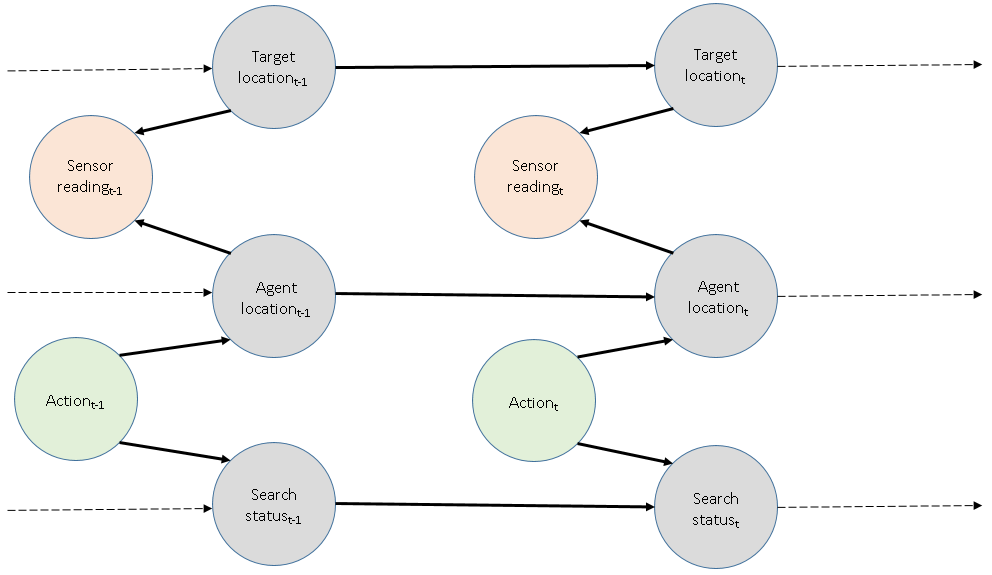
\includegraphics[width = 0.8\linewidth]{Chapters/MultiAgentTargetDetection/Figs/DBNWithMultipleHiddenState.PNG}
     \caption{First Version of the DBN representing the agent world model}
    \label{fig:FirstDBNUsed}
\end{figure}
A number of conditional probabilities are specified here in order to describe the factored joint distribution of the world model fully. The full tables are omitted as they are sparse. For brevity, we use the abbreviation Loc for Location.



\begin{figure}[H]
\scriptsize
\begin{equation}\label{eqn:EvidenceVarsProbs}
    %\centering
    p(SensorReading_t | AgentLoc_{t-1}, EvidenceLoc_{t-1})  = 
    \begin{cases}
    \alpha \quad \text{ if } SensorReading_t=1 \text{ and } EvidenceLoc_t \neq AgentLoc_t
    \\
    1-\beta \quad \text{ if } SensorReading_t=1 \text{ and } EvidenceLoc_t = AgentLoc_t
    \\
    \beta \quad \text{ if } SensorReading_t=0 \text{ and } EvidenceLoc_t \neq AgentLoc_t
    \\
    1-\alpha \quad \text{ if } SensorReading_t=0 \text{ and } EvidenceLoc_t \neq AgentLoc_t
    \end{cases}
    %
\end{equation}
\caption{Conditional Probability Distribution for the $Evidence$ Variable}
\end{figure}


\begin{figure}[H]
\scriptsize
\begin{equation}\label{eqn:TargetLocProbs}
    p(TargetLoc_{t} | TargetLoc_{t-1}) =
    \begin{cases}
    1 \quad \text{ if } TargetLoc_{t}=TargetLoc_{t-1}
    %agent returns correct target Loc.} 
    \\
    0 \quad \text { otherwise. }
    \end{cases}
\end{equation}
\caption{Conditional Probability Distribution for the $TargetLocation$ Variable}
\end{figure}





\begin{figure}[H]
\scriptsize
%\begin{equation}\label{eqn:SearchStatus}
    \begin{gather}\label{eqn:SearchStatus}
        p(SearchStatus_t | SearchStatus_{t-1}, Action_{t-1}) = \\
        \begin{cases}
        1 \quad \text{ if } SearchStatus_t = terminated\_x_i \text{ and } SearchStatus_{t-1} = terminated\_x_i 
        \\
        1 \quad \text{ if } Action_t = terminate\_x_i \text{ and } SearchStatus_{t-1}=ongoing \text{ and } SearchStatus_{t} = terminated\_x_i
        \\
        1 \quad \text{ if } Action_t = move\_x_i \text{ and } SearchStatus_{t-1}=ongoing \text{ and } SearchStatus_t=ongoing
        %agent returns correct target location.} 
        \\
        0 \quad \text { otherwise. }
        \end{cases}
    \end{gather}
%\end{equation}
\caption{Conditional Probability Distribution for the $SearchStatus$ Variable}
\end{figure}





\begin{figure}[H]
\scriptsize
    \begin{equation}\label{eqn:AgentLocation}
        p(AgentLoc_t | AgentLoc_{t-1}, Action_{t}) = 
        \begin{cases}
        1 \quad \text{ if } Action_t = move\_x_i \text{ and } AgentLoc_t = x_i
        \\
        1 \quad \text{ if } Action_t = terminate\_x_i \text{ and } AgentLoc_t = AgentLoc_{t-1}
        \\
        0 \quad \text{otherwise}
        \end{cases}
    \end{equation}
\caption{Conditional Probability Distribution for the $AgentLocation$ Variable}
\end{figure}


\normalsize
The semantics of the equations listed above is given here: 
\begin{enumerate}
    \item Equation \ref{eqn:EvidenceVarsProbs} uses two parameters, $\alpha$ and $\beta$, to represent the probability of making a false positive and false negative sensor reading, respectively. These are assumed to have been calculated by using pre-calibrated values of the sensor. This model is very flexible and does not stipulate any restrictions on the sensor other than that it must return a reading indicating that the target is present or not.
    \item  Equation \ref{eqn:TargetLocProbs} simply states that the location of the target does not change, even though it is hidden. It would be very easy to modify this to allow for moving target detection in the case of a non-static target.
    \item Equate \ref{eqn:SearchStatus} is also states a number of intuitive notions. The first line states that once the agent terminates the search, it remains over. The second line states that if the agent requests an ongoing search to terminate, then it does so deterministically. The third line states that if the agent chooses to move in an ongoing search, then the search remains ongoing.
    \item Equation \ref{eqn:AgentLocation} simply outlines that the agent moves to new locations deteministically. It also indicates that should the agent choose to terminate the search, then the environment enters a terminal state, indicating that the search is over.
\end{enumerate}


Note that despite the fact that some hidden state variables cannot be observed directly, it is still possible to infer their value exactly based on their starting state. For example, the position of the agent is a deterministic function of its actions and previous position. These variables could have been treated as variables that are internal to the agent rather than part of the hidden world state and many authors omit such variables for the sake of clarity.
\note{need to outline why I have included them - mainly because evidence probability depends on agent location as well as source location}


\subsubsection{Estimated State}
\workinprogress
Since the agent operates in a partially observable environment, the agent's internal state representation of the environment needs to take into account the fact that the current environment state is not certain. For this reason, a probability distribution over possible environment states is used by the agent to internally represent the environment state. The internal agent state is described mathematically by 
\[p(x_t | e_{1:t}, u_{1:t})\]
, which is the distribution of possible world states given all evidence and control actions up to the current time step, where $x_t$, $e_t$ and $u_t$ follow the conventions of being the hidden state variables, the evidence variables and the control action variables. The agent updates this state using the world model specified in the preceding chapter, using the filtering algorithm explained in section \ref{subsection:InferenceHMMDBN} of Chapter \ref{chapter:Background}. There are a couple of noteworthy points:
\begin{itemize}
    \item A distribution that has a single sharp peak would indicate that the agent believes that the target is at a specific location with high confidence. This is clearly preferred to a flat, uniform distribution representing uncertainty in relation to where the target might be.
    \item The only true source of uncertainty in the world state is introduced by the sensor. Therefore, analysis of this state representation in relation to the sensor model should provide insight into how the system performs.
\end{itemize}
In order to update the estimated state of the agent, the below equations are used, which are described in subsection \ref{subsection:InferenceHMMDBN}. For brevity $x_t$ denotes the hidden state variables, $e_t$ denotes the evidence variable and $u_t$ denotes the control action taken by the agent. The equations only describe the estimated state update for move actions, since if the agent terminates the search a terminal state is deterministically entered. The $SearchStatus$ variable is omitted from the equations since it only effects the equations if the $Action$ variable is to terminate the search.
\footnotesize
\begin{figure}[H]
\scriptsize
%\begin{equation}\label{eqn:SearchStatus}
    \begin{gather}\label{eqn:SearchStatus}
        p(AgentLoc_t = x, TargetLoc_t = y | e_{1:t}, u_{1:t}) = \\
        \begin{cases}
            \eta \alpha p(AgentLoc_{t-1} = x, TargetLoc_t = y | e_{1:t-1}, u_{1:t-1}) \text{ if $e_t$ is a positive reading and $AgentLoc_t \neq TargetLoc_t$} \\
            \eta \beta p(X_{t-1}=x_t | e_{1:t-1}, u_{1:t-1}) \text{ if $e_t$ is a negative reading and $Agent_loc_t$ = $TargetLoc_t$} \\
            \eta (1-\alpha) p(X_{t-1}=x_t | e_{1:t-1}, u_{1:t-1}) \text{ if $e_t$ is a negative reading and $Agent_loc_t \neq TargetLoc_t$} \\
            \eta (1-\beta) p(X_{t-1}=x_t | e_{1:t-1}, u_{1:t-1}) \text{ if $e_t$ is a positive reading and $Agent_loc_t$ = $TargetLoc_t$} \\
        \end{cases}
%\eta O_{t} T^{T} f_{1:t-1} 
    \end{gather}
\end{figure}
\normalsize

\subsubsection{Action Selection Strategy}
\workinprogress
At each time step the agent may either choose to terminate the search or move to a new location to take a measurement reading. The agent may choose which of these actions to perform based on its location, the search status and its internal representation of the environment, which are outlined in the preceding section. First we discuss how move actions are chosen, if the agent decides that the search should not be terminated at the current time step. We began by implementing some of the recommended basic search strategies outlined in the related works by \citeauthor{Chung2007ASearchb} \cite{Chung2007ASearchb} and \citeauthor{Waharte2010SupportingRAVs} \cite{Waharte2010SupportingRAVs}. These search methods are devised in order to optimize the agent's performance measure, which is set out in \ref{sssection:PerfMeas}. The results of applying these strategies are discussed in <give reference to results section>\par 
\note{In the following, might be good to mention the motivation in relation to the performance measure}
\textbf{Random Search}
This method serves as a baseline against which similar strategies can be compared. The agent simply chooses the next grid location to explore randomly from all possible grid locations. The expected number of moves needed to take a reading at all possible grid cells is given by the solution to the well-known \textit{coupon collectors problem}, $nH_n$, where $H_n$ is the $n_{th}$ harmonic number and $n$ is the total number of grid cells, which gives a good idea of the expected amount of time that will be taken to conclude the search.

\textbf{Greedy Search}
A simple greedy search was implemented next, where the agent chooses to visit the grid cell with the highest estimated probability of containing the target in a localized region around the agent:
\footnotesize
\[
Action_t = \argmax_{NewLoc \in N(AgentLoc)}{p(TargetLoc = NewLoc, SearchStatus, AgentLocation| e_{1:t}, u_{1:t})}
\]
\normalsize
$N(AgentLoc)$ is a function that returns a neighborhood of locations around the agent's location and can be calibrated to trade off the cost of saccading between grid cells that may be far from each other against the cost of limiting the agents range to a narrow and possible "cold" region.This method is designed bearing in mind that there may be motivation to explore some areas before others based on prior knowledge. 

%\textbf{$\epsilon$-greedy Search} Greedy search  simplest method to implement was an $\epsilon$-greedy action selection method, whereby the agent moves to the grid cell with the highest estimated probability in a pre-defined radius with probability 1-$\epsilon$ and a random grid cell in the pre-defined with probability $\epsilon$. This encourages the agent to exploit it's current know\par

\textbf{Sweep Search}
This strategy sweeps the region of interest systematically, aiming to take a reading at each grid cell an equal number of times while minimizing the total distance travelled. It then traverses this same path again in reverse order. This required planning a trajectory in advance, which is often referred to in related literature as the \textit{complete coverage path}. Since the region to be swept is assumed to be a grid, where adjacent points are assumed to be equidistant, a number of heuristic solutions were explored which are outlined in section <reference to route planning>.\par

\textbf{POMDP Based Search} 
\note{Not sure if I should go into this at all. Work was done in understanding POMDPs and clearly the solution can be easily framed as a POMDP but my work stopped short in actually finding a solution to POMDP that works well}
As outlined in 
details. \par

\subsection{Search Cutoff Strategy}


\workinprogress

At each discrete timestep, the agent can either choose to move to a new grid location to record a sensor measurement or it can decide to terminate the search based on its estimated state of the environment. There is a trade-off in terminating the search early, which means that less time and resources are spent on continuing the search, versus the possibility of drawing misinformed conclusions from the search due to a lack of information. For example, if the agent receives a series of false positive readings at a given location, it could mistakenly choose to conclude that the target is present at a given location rather than sample further to gain confidence that it has correctly found the location of the target. Following this line of thinking, it is clear that a strategy needs to be devised to minimize the probability of drawing false conclusions, which is in line with the performance measure set out in \ref{sssection:PerfMeas}.\par
Previous related work, \cite{Chung2007ASearchb} has addressed this problem using methods that use heuristics as well as a more formal asymptotic theory-based approach. We ultimately choose to implement the Sequential Probability Ratio Test (SPRT), which is a hypothesis-testing framework developed by \citeauthor{Wald1950BayesProblems} to optimally deal with sequential decision problems, as opposed to traditional frameworks which assume that all the necessary data has been gathered prior to analysis \cite{Wald1950BayesProblems}. The details of the proof of optimality of the SPRT is given in \cite{Wald1950BayesProblems} and we have outlined the details of how to perform hypothesis-testing using this framework in section <refer to the section>, along with the practical advantages and drawbacks of using it. In order to allow the agent to make a decision on whether to terminate the search or not, the following procedure was used: \note{Might be worthwhile simply outlining the algorithm}
\begin{gather}\label{eqn:SearchStatus}
H_0 : \text{The target is not present in the search region}
\\
H_1 : \text{The target is present in the search region}
\end{gather}\label{searchTermination}
\note{Some of this could be moved to background}



\subsubsection{Implementing the Agent}
\placeholder

\subsubsection{Initial Results}
\placeholder

\subsection{Incorporating Battery Capacity Constraints}
\placeholder

\subsubsection{Incorporating Multiple Targets}
\placeholder

\subsubsection{Incorporating Multiple RAVs}
\placeholder



\begin{enumerate}
    \item How to design the agent function, as discussed in chapter \ref{Background}.
    \item What kind of model can be used to describe the agent's environment (assuming using a model-based, utility-based agent function design).
    \item What kind of internal state does the agent need to maintain.
    \item When should the agent cutoff its search for the target?
    \item How should the agents choose actions to perform based on its model of the environment?
    \item What percepts will the agent receive and what actions will it perform? How can these be represented using software?
\end{enumerate}

The target detection problem described in this thesis naturally decomposes into a number of sub-problems. %These components aren't independent, might be worth discussing how the components interact.

One component is obviously the world model, which is the agent's internal representation of the world and it's dynamics. The agent maintains an internal state
\subsubsection{Results}
%How to break this down - by control strategy, problem type etc.?

\subsection{Discussion and Conclusions}
\subsubsection{Limitations}
%Talk about  problem of grid resolution, drift may be an issue if GPS not present (this could be addressed by assuming that an initial mapping phase is carried out, so mapping is all that's necessary to keep track of location while searching)